\documentclass[12pt]{report}			% Začátek dokumentu
\usepackage{MP}				
\usepackage{amsmath}
\usepackage{mathtools}
\usepackage{graphicx}		% Import stylu
\usepackage{indentfirst}
\author{David Kolář}
\title{Geometrická posloupnost a posloupnosti z ní odvozené}
\date{14. února 2023}
\vedouci{Mgr. Michaela Petrová}
\place{V Českých Budějovicích}
\skolnirok{2022/2023}
\logo{
\includegraphics[scale=1.25]{GJ8_logotyp}}
\makeatletter
\newcases{centercases}{\quad}
  {\hfil$\m@th\displaystyle{##}$\hfil}
  {$\m@th\displaystyle{##}$\hfil}{\lbrace}{.}
\makeatother

\begin{document}
\pagenumbering{roman}                   % číslování stránek římskými číslicemi
	\mytitlepage						% Vygenerování titulní strany
	
	\prohlaseni{
		Prohlašuji, že tato maturitní práce je mým původním autorským dílem, které jsem vypracoval samostatně. Všechny zdroje, prameny a literaturu, které jsem při vypracování
používal nebo z nich čerpal, v práci řádně cituji s uvedením úplného odkazu na příslušný
zdroj.

	}	
	
	\abstrakt{
	
				% Abstrakt
	}{
							% Klíčová slova
	}
	
	\podekovani{
Rád bych vyjádřil hlubokou vděčnost vedoucí mojí práce, paní Michaele Petrové, za její neocenitelné vedení, mnoho užitečných rad a hlavně za její trpělivost. 
Dále bych rád poděkoval svému dobrému příteli Lukáši Knotovi, velkému zdroji inspirace, za poskytnutí nového pohledu na mou práci, konstruktivní kritiku a zpětnou vazbu.				% Poděkování
	}
	
   {\tableofcontents\newpage}			% Obsah
	
\addtocounter{page}{1}		% Posunutí countru stránek
\pagenumbering{arabic}		% Číslování stránke arabskými číslicemi
	\chapter*{Úvod}
Vždy mě fascinovaly matematické posloupnosti a jejich součty, a proto jsem se rozhodl na toto téma zpracovat svou maturitní práci. V matematice a informatice se při určování časové a prostorové složitosti algoritmu často spoléháme na vyhodnocení právě součtu členů posloupností. Proto může být nalezení uzavřeného tvaru, neboli součtového vzorce posloupnosti, nesmírně užitečné.

Moje maturitní práce je rozdělena na dvě části: teoretickou část a praktickou část. 
V teoretické části začnu definicí toho, co je to matematická posloupnost a pojednám o jejích různých typech a vlastnostech. Poté se budu věnovat specifickým vlastnostem geometrické a aritmetické posloupnosti, včetně jejich součtových vzorců, a ukážu uplatnění geometrické posloupnosti při určování časové a prostorové složitosti. Dále představím pojem aritmeticko-geometrické posloupnosti a vysvětlím, čím se liší od ostatních typů posloupností. Nakonec ukážu svou vlastní posloupnost, kterou jsem objevil při studiu.

V praktické části své práce uvedu důkaz součtu geometrické, aritmeticko-geometrické a mojí posloupnosti. 

Celkově si má maturitní práce klade za cíl poskytnout základní přehled týkající se matematických posloupností, konkrétně geometrické, aritmeticko-geometrické a mojí posloupnosti a představit mé poznatky a myšlenky na toto téma.

	
	
	\part{Teoretická část}
	
		\chapter{Zavedení pojmu posloupnost}
		
			
			\section{Definice a vysvětlení pojmu funkce}
Pro zavedené pojmu posloupnost je nutné nejprve zavést a vysvětlit obecnější pojem funkce. V matematice označuje pojem funkce vztah mezi množinou vstupů a množinou výstupů s vlastností, že každému vstupu je přiřazen právě s jeden výstup. Vstup funkce se nazývá argument a výstup se nazývá hodnota funkce.

Funkce jsou důležitým nástrojem v matematice a používají se v mnoha různých oblastech, včetně fyziky, inženýrství, ekonomie a dalších. Lze je analyzovat pomocí různých matematických technik jako je infinitezimální počet a algebra. Nejprve zavedeme základní pojmy týkající se funkcí.


				\paragraph{Definice 1 [Funkce]:}
 Funkce na množině $\mathbb{D} \subset \mathbb{R}$ je předpis, který každému číslu z množiny  $\mathbb{D}$ přiřazuje právě jedno reálné číslo.

				\paragraph{Definice 2 [Definiční obor]:}
Pokud máme funkci $f$, pak množině $D$, na které je funkce $f$ definována, se říká \emph{definiční obor} funkce $f$ a značí se $D(f)$.
		\paragraph{Definice 3 [Obor hodnot]:}
Obor hodnot je množina všech reálných čísel $y$, která lze dostat jako výstupní hodnotu funkce $f$, jestliže se za $x$ dosadí všechny přípustné hodnoty z $D(f)$. Obor hodnot funkce $f$ se značí $H(f)$.
\newpage
				\subsection{Zadání funkce}
Funkci lze zadat několika způsoby, ty nejvýznamnější si ukážeme na funkci $\sin(x)$.

					\subsubsection{Předpisem}
					\begin{itemize}
					\item $f:\quad y = \sin(x)$
					\item $y = \sin(x)$
					\item $x \to \sin(x)$
					\end{itemize}
Toto vše jsou validní notace předpisu funkce. Při používání předpisu je nezbytné určit definiční obor.
				\subsubsection{Tabulkou}
První řádek představuje vstup funkce $x$ a druhý řádek výstup funkce $sin(x)$.
\begin{center}
\begin{tabular}{ | m{1cm} | m{1cm}| m{1cm} | m{1cm} |m{1cm} |m{1cm} |} 
\hline
  $x$ & $0$ & $\frac{\pi}{6}$ & $\frac{\pi}{4}$ & $\frac{\pi}{3}$ & $\frac{\pi}{2}$ \\
\hline
	$\sin(x)$ & $0$ & $\frac{1}{2}$ & $\frac{\sqrt{2}}{2}$ & $\frac{\sqrt{3}}{2}$ & $1$ \\
\hline
\end{tabular}
\end{center}
				\subsubsection{Grafem}
Graf funkce $\sin(x)$ s oborem definice $D(f) = \langle 0, 2\pi \rangle$. Pro vizualizaci jsem použil program Geogebra.
\begin{center}
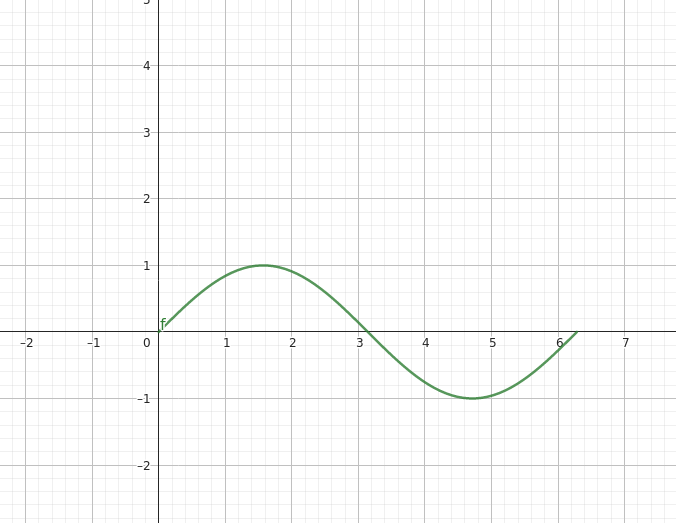
\includegraphics[scale=0.4]{./images/graf.png}
\end{center}

		\section{Vysvětlení pojmu posloupnost}
Posloupnost je funkce definovaná na množině přirozených čísel\footnote{Někdy se posloupnosti indexují od $0$. Pro přehlednost jsem se ale rozhodl ponechat v teoretické části jen indexování od $1$.}, což jsou celá kladná čísla (1, 2, 3 atd.). Stejně jako u funkce tedy platí, že se jedná o vztah mezi množinou vstupů a množinou možných výstupů s vlastností, že ke každému vstupu je přiřazený právě jeden výstup. Definiční obor posloupnosti může být buď konečná množina, pak se posloupnost nazývá \emph{konečná}, nebo \emph{nekonečná} množina, pak se posloupnost nazývá \emph{nekonečná}.
		\section{Značení}
Prvky z definičního oboru posloupnosti $(a_n)$ budu označovat $n$ a funkční hodnoty posloupnosti $(a_n)$ označovat $a_n$. Platí tedy, že $n$-tému prvku je přiřazena hodnota $a_n$.
		\subsection{Značení nekonečné posloupnosti}
Nekonečné posloupnosti budu značit $(a_n)_{n=1}^{\infty} $.
		\subsection{Značení konečné posloupnosti}
Konečné posloupnosti budu značit jako $(a_n)_{n=1}^k$ kde přirozené číslo $k$ označuje maximální velikost $n$. Definiční obor posloupnosti $(a_n)$ tedy zahrnuje všechna přirozená čísla od $1$ do $k$. 

Zápisem ve tvaru $n \in \{1, \dots, k\}$ vyjadřuji, že $n$ nabývá hodnotu všech přirozených čísel od $1$ do $k$.

\section{Zadání posloupnosti}
Posloupnost lze zadat různými způsoby v závislosti na povaze posloupnosti, potřebách dané situace a preferencích osoby, která je používá.

Jedním ze způsobů vyjádření posloupnosti je rekurentní vzorec, který definuje každý člen posloupnosti pomocí jeho předchozích členů. 

Dalším způsobem vyjádření posloupnosti je pomocí vzorce, který definuje $n$-tý člen posloupnosti an pomocí proměnné $n$. Tento způsob může být užitečný třeba pro posloupnosti, které mají jednoduchý vzorec a lze je snadno definovat. To platí například pro aritmetickou nebo geometrickou posloupnost. 
Konečnou posloupnost lze vyjádřit výčtem hodnot:
\[(a_n)_{n=1}^k=[1, 4, 9, 16, 25]\]  
\newpage
Dále lze zadat konečnou posloupnost graficky. Tato metoda je užitečná pro vizualizaci posloupnosti, neboť s ní lze posloupnost lépe pochopit a interpretovat.
\begin{center}
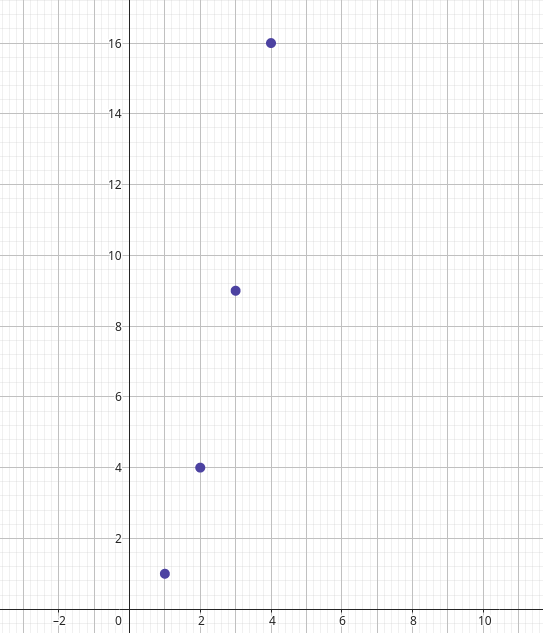
\includegraphics[scale=0.4]{./images/graf_posloupnosti.png}

\end{center}
Poslední ze základních metod, jakou lze zadat konečnou posloupnost je s pomocí tabulky:


\begin{center}
\begin{tabular}{ | m{1cm} | m{1cm}| m{1cm} | m{1cm} |m{1cm} |m{1cm} |} 
\hline
  $n$ & $1$ & $2$ & $3$ & $4$ & $5$ \\
\hline
	$a_n$ & $1$ & $4$ & $9$ & $16$ & $25$ \\
\hline
\end{tabular}
\end{center}

\subsection{Vzorec pro $n$-tý člen}
Vzorcem pro $n$-tý člen lze zadat posloupnost konečnou i nekonečnou.
Vzorec pro $n$-tý člen vyjadřuje vztah mezi hodnotou $n$ z definičního oboru a $a_n$ z oboru hodnot. Dosazením hodnoty $n$ do tohoto vzorce lze zjistit $n$ -tý člen an posloupnosti.
\subsubsection{Příklady:}
Nekonečnou posloupnost lze zapsat několika způsoby:
\[a_n = 2n + 1 \]

Tento zápis nápadně připomíná formu zápisu funkce. Druhý způsob už se více blíží zápisu posloupností, jak jsme si jej definovali dříve.
\[(2n + 1)_{n=1}^{\infty} \]

Konečnou posloupnost, kde $n \le k$ potom lze zapsat kupříkladu takto:
\[(2n + 1)_{n=1}^{k} \]
\[a_n = 2n + 1 \quad n \le k \quad n \in \mathbb{N}\]
\subsection{Rekurentní vzorec}
Rekurentní vzorec určuje člen posloupnosti pomocí znalosti jednoho nebo více předcházejících členů. Tento způsob je užitečný zejména u posloupností, které mají složitý předpis a nelze je snadno definovat pomocí jediného vzorce. Známým příkladem je Fibonacciho posloupnost.
\subsubsection{Příklad na Fibonacciho posloupnosti:}
Fibonacciho posloupnost, poprvé popsána v indické matematice již 200 let př. n. l., je posloupnost čísel, ve které je každé číslo, kromě prvních dvou čísel,$0$ a $1$, součtem dvou předchozích, tedy $0, 1, 1, 2, 3, 5, 8, 13, 21$ atd. 
\[
a_{n}=
\begin{centercases}
  0         & n=1 \\
  1 		   & n=2 \\
  a_{n-1}+ a_{n-2}& n>2
\end{centercases}
\]
Tato posloupnost je sice nekonečná, nicméně pomocí rekurentního vzorce lze zadávat i konečné posloupnosti. Ukážeme si to opět na předchozím příkladu:
\[
a_{n}=
\begin{centercases}
  0         & n=1 \\
  1 		   & n=2 \\
  a_{n-1}+ a_{n-2}& 2<n\le10
\end{centercases}
\]
\section{Vlastnosti posloupností}
Protože je posloupnost definovaná jako funkce s definičním oborem přirozených čísel,  lze mnoho vlastností, které platí pro funkce obecně, určit i pro posloupnosti, například monotónnost nebo omezenost.
\subsection{Monotónnost posloupnosti}
Jednou z vlastností, kterou lze pro posloupnost určit, je monotónnost, která se týká rostoucí nebo klesající povahy jednotlivých prvků.
\paragraph{Definice 4 [Rostoucí posloupnost]:}
O posloupnosti se říká, že je rostoucí, jestliže je každý člen větší než předchozí.

\begin{equation}
\forall n,m \in D:n<m \Rightarrow a_n < a_m
\end{equation}

\paragraph{Definice 5 [Klesající posloupnost]:}
Posloupnost je klesající, jestliže je každý člen menší než předchozí člen.

\begin{equation}
\forall n,m \in D:n<m \Rightarrow a_n > a_m
\end{equation}

\paragraph{Definice 6 [Nerostoucí posloupnost]:}
O posloupnosti se říká, že je nerostoucí, jestliže je každý člen menší nebo roven předchozímu členu.

\begin{equation}
\forall n,m \in D:n<m \Rightarrow a_n \geq a_m
\end{equation}

\paragraph{Definice 7 [Neklesající posloupnost]:}
O posloupnosti se říká, že je neklesající, jestliže je každý člen větší nebo roven předchozímu členu.

\begin{equation}
\forall n,m \in D:n<m \Rightarrow a_n \leq a_m
\end{equation}
\paragraph{Definice 8 [Nerostoucí posloupnost:]} O posloupnosti se říká, že je nerostoucí, jestliže je každý člen menší nebo roven předchozímu členu. Posloupnost $(a_n)$ se nazývá nerostoucí právě tehdy, když: 
\begin{equation}
\forall n,m \in D: n < m \Rightarrow a_n \geq a_m.
\end{equation}
\paragraph{Definice 9 [Neklesající posloupnost]:} O posloupnosti se říká, že je neklesající, jestliže je každý člen větší nebo roven předchozímu členu. Posloupnost $(a_n)$ se nazývá neklesající právě tehdy, když:
\begin{equation}
\forall n,m \in D: n < m \Rightarrow a_n \leq a_m
\end{equation}
\subsection{Omezenost posloupnosti}
Další vlastností, kterou lze u posloupnosti určit, je omezenost, která se týká maximálních a minimálních hodnot, kterých mohou členy nabývat a neomezená, pokud žádná taková hranice neexistuje. To je třeba opravit.
\paragraph{Definice 10 [Shora omezená]:}
Posloupnost $(a_n)$ je shora omezená, jestliže existuje $h \in \mathbb{R}$ takový, že pro všechny $n \in D$ platí $a_n \leq h$.

\paragraph{Definice 12 [Zdola omezená]:}
Posloupnost $(a_n)$ je zdola omezená, jestliže existuje $d \in \mathbb{R}$ takový, že pro všechny $n \in D$ platí $a_n \geq d$.

\paragraph{Definice 12 [Omezená]:}
Posloupnost $(a_n)$ je omezená, jestliže je shora i zdola omezená, tedy existují $h,d \in \mathbb{R}$ takové, že pro všechny $n \in D$ platí $d \leq a_n \leq h$.
\chapter{Řady}

Řada vznikne sečtením prvků posloupnosti. Pokud je posloupnost konečná, vznikne konečná řada, pokud je posloupnost nekonečná, vznikne sečtením jejích členů nekonečná řada. V textu jsem se zatím pojmu řada vyhýbal, i když by mohl být na mnoha místech užitečný, takže ho postupně do textu zařadím.

\section{Definice}

Je dána posloupnosti $(a_n)$. Výraz tvaru
\begin{equation}
a_1 + a_2 + a_3 + \dots + a_n + \dots
\end{equation}
je řada.

\section{Konvergentní a divergentní řady}

\paragraph{Definice 12 [Konvergentní řada]:}
Řada se nazývá konvergentní, pokud je její součet reálné číslo. 
\paragraph{Definice 13 [Divergentní řada]:}
Řada se nazývá divergentní, pokud její součet není reálné číslo. 

\chapter{Aritmetická posloupnost}

Aritmetická posloupnost je posloupnost čísel, ve které je rozdíl mezi dvěma po sobě jdoucími členy vždy stejný. Tento společný rozdíl může být kladný, záporný nebo nulový a určuje rychlost změny posloupnosti a zda je posloupnost konstantní, rostoucí, či klesající.

\paragraph{Definice 14 [Aritmetická posloupnost]:}

Posloupnost $(a_n)$ se nazývá aritmetická právě tehdy, když $\exists d \in \mathbb{R} \ \forall n \in \mathbb{N}$ a platí, že $a_{n+1} = a_n + d$


\section{Vyjádření pomocí vzorce}

Aritmetická posloupnost se často vyjadřuje pomocí následujícího vzorce:
\begin{equation}
a_n  = a(1) + (n-1)d,
\end{equation}
kde $a(n)$ je $n$-tý člen posloupnosti, $a(1)$ je první člen a $d$ je rozdíl dvou po sobě jdoucích členů. \section{Součet}
Součet prvních n členů aritmetické posloupnosti lze vyjádřit jako:
\begin{equation}
s_n=n\frac{a_1+a_n}{2}
\end{equation}

kde $a_1$ označuje první prvek a $a_n$ poslední.

\chapter{Geometrická posloupnost}
Geometrická posloupnost je posloupnost, kde je každý člen kromě prvního násobkem předchozího členu. Tento násobek, označovaný jako základ či kvocient může být kladný, záporný nebo nulový a určuje směr a rychlost změny posloupnosti.
Geometrické posloupnosti nachází uplatnění v různých matematických souvislostech a lze je použít k modelování reálných jevů, které vykazují exponenciální růst nebo pokles, třeba ekonomický růst nebo šíření viru. Běžně se používají také v informatice, zejména při analýze algoritmů a datových struktur, kde se využívá například vztah pro součet nekonečné posloupnosti se základem $|q| < 1$. Tomuto uplatnění se budu věnovat později. 

\paragraph{Definice 16 [Geometrická posloupnost:}
Posloupnost $(an)$ se nazývá geometrická právě tehdy, když: 
$$\exists q \in \mathbb{R} \forall n \in \mathbb{N}, a_{n+1} = a_n \cdot q$$
\section{Vyjádření pomocí vzorců}
Geometrická posloupnost se často znázorňuje pomocí následujícího vzorce:

$$a_{n} = a_{1} \cdot q^{n-1}$$

kde $a_{n}$ je n-tý člen posloupnosti, $a_{1}$ je první člen a $q$ je základ.
Součet prvních $n$ členů geometrické posloupnosti se vyjádřuje jako:

$$s_n = \frac{a_1 (q^n - 1)}{q-1}$$

Odvození tohoto tvrzení bude poskytnuto v praktické části maturitní práce. Pokud platí, že $|q| < 1$, pak se součet pro $n$ se blížící nekonečnu limitně blíží k: $$\frac{a_1}{1-q}$$.
\section{Určení asymptotické složitosti pomocí geometrické posloupnosti}
Součet některých konvergujících geometrických posloupností nachází uplatnění třeba při určování časové složitosti algoritmu. Například při konstrukci haldy v $O(n)$\footnote{Pro vstup o délce $n$ potřebuje program řádově $n$ kroků k doběhnutí.}, při dynamickém zvětšování a zmenšování pole\supercite{1} nebo hashovací tabulky\cite{1} či u algoritmu Quickselect\cite{1} používaný k nalezení $k$-tého nejmenší prvku v poli, který má v průměru lineární časovou složitost.
\chapter{Aritmeticko-geometrická posloupnost}
Posloupnost aritmeticko-geometrická je posloupnost $a_1 b_1, a_2 b_2, \ldots, a_n b_n$, kde posloupnost $a_1, a_2, \ldots, a_n$ je aritmetická a posloupnost $b_1, b_2, \ldots, b_n$ geometrická.
\paragraph{Definice 16 [Aritmeticko-geometrická posloupnost]:}
Posloupnost $(a_n)$ se nazývá aritmeticko-geometrická právě tehdy, když:
$$a_n = (a + d(n-1)) \cdot bq^n, \quad n\in\mathbb{N}, \quad a,b,q\in\mathbb{R}.$$
\section{Součtový vzorec}
Součet prvních $n$ prvků Aritmeticko-geometrické posloupnosti lze zapsat ve formě vzorce:
$$s_n = \frac{a+dq\frac{1 - q^n}{1 - q} - (a + nd)q^n}{1-q}$$
Součet odvodím ve svojí praktické části.
\chapter{Obecná posloupnost ve tvaru součinu \\ polynomu a exponenciály}
Při studiu geometrické a aritmeticko-geometrické posloupnosti jsem si uvědomil, že lze stejné schéma odvození součtového vzorce prvních $n$ prvků uplatnit i na libovolnou posloupnost ve tvaru $a_n = (n-1)^kq^{n-1}$, kde $k$ je libovolné nezáporné celé číslo. Nadefinoval jsem si tedy $a$ a sečetl prvních $n$ prvků posloupnosti ve tvaru $a_n = a\cdot p(n-1)\cdot q^{n-1}$, kde $p(n-1)$ představuje libovolný polynom. V závěru praktické části maturitní práce představím odvození rekurentního vztahu pro určení součtového vzorce prvních $n$ prvků posloupnosti $a_n = (n-1)^kq^{n-1}$ a využiji pravidla distributivnosti, se kterým demonstruji, jak lze tento rekurentní vztah využít pro součet prvních $n$ prvků posloupnosti tvaru $a\cdot p(n-1)\cdot q^{n-1}$.
\part{Praktická část}
\section*{Odvození vztahu}

{\bf Značení:} Uvažujme \(e\), kde \(e \in \mathbb{Z}_{\geq 0}\). Pak \(\prescript{e}{}{a_i}\) je člen posloupnosti ve tvaru \(i^eq^i\) a  \(\prescript{e}{}{s_n} = \sum_{i = 0}^{n} \prescript{e}{}{a_i}\)\\\\\
{\bf Věta 1:} Nechť \(q \in \mathbb{R}\setminus\{1\}\) \[\prescript{1}{}{s_n} = \frac{q}{q - 1}(nq^{n}+q^{n} - \frac{q^{n+1}-1}{q-1})  \]
{\bf Lemma:} \[\prescript{0}{}{s_n} = \sum_{i=0}^{n} q^{i}=\frac{q^{i+1} - 1}{q - 1}\]
Z definice platí, že: \begin{equation} \prescript{0}{}{s_{n+1}} = \prescript{0}{}{s_{n}} + q^{n+1}\end{equation}\\Dále uvedu ještě jeden vztah mezi \(\prescript{0}{}{s_{n+1}}\) a \(\prescript{0}{}{s_{n}}\), který již není tolik zřejmý. Vynasobením každého členu \(\prescript{e}{}{a_i}\) koeficientem \(q\) získám člen o stupeň větší, neboť platí:
\[\prescript{0}{}{a_{n}}q=q^iq=q^{i+1}=\prescript{0}{}{a_{n+1}}\]Tím vytvořím posloupnost \(\prescript{0}{}{a_{1}}\dots\prescript{0}{}{a_{n+1}}\). Příčtením \(\prescript{0}{}{a_0}\) mi tedy vznikne posloupnost \(\prescript{0}{}
{a_0}\dots\prescript{0}{}{a_{n+1}}\)
a tudíž platí, že:
\[\prescript{0}{}{s_{n+1}} = \prescript{0}{}{s_{n}}q + 1\]
Dosadím vztah (1):
\[\prescript{0}{}{s_n} + q^{n+1} = \prescript{0}{}{s_{n}}q + 1\]
Vyjádřím si \(\prescript{0}{}{s_n}\) a získám námi hledaný tvar.
\[\prescript{0}{}{s_{n}} =\frac{q^{n+1} - 1}{q - 1}\]
{\it Důkaz:}\\\\Budu postupovat podobně jako v lemmatu. Z definice platí: \begin{equation} \prescript{1}{}{s_{n+1}} = \prescript{1}{}{s_{n}} + (n+1) q^{n+1}\end{equation}
Mějme posloupnost \(\prescript{1}{}{a_{0}}\dots\prescript{1}{}{a_{n}}\).
Ke každému členu \(\prescript{1}{}{a_{i}}\) přičtu odpovídající \(\prescript{0}{}{a_{i}}\). Takto získám novou posloupnost, kde každý člen odpovídá tvaru: \((x+1)q^x\). Náhlednu, že vynásobením členu \(q\) získám člen \(\prescript{1}{}{a_{i+1}}\).
\[q(\prescript{1}{}{a_{i}}+\prescript{0}{}{a_{i}})=\prescript{1}{}{a_{i+1}}\]
Z čehož plyne:
\[\prescript{1}{}{s_{n+1}}=q(\prescript{1}{}{s_{n}} + \prescript{0}{}{s_{n}})\]
Dosadím si vztahy (1), (2):
\[\prescript{1}{}{s_{n}} + (n+1) q^{n+1}=q(\prescript{1}{}{s_{n}} + \frac{q^{n+1} - 1}{q - 1})\]
Vyjádřím si \(\prescript{1}{}{s_{n}}\).
\[\prescript{1}{}{s_{n}}=\frac{(n+1) q^{n+1} - q(\frac{q^{n+1} - 1}{q - 1} )}{q - 1}\]
Výsledný vztah upravím na námi hledaný tvar:
\[\prescript{1}{}{s_n} = \frac{q}{q - 1}(nq^{n}+q^{n} - \frac{q^{n+1}-1}{q-1})  \]
{\bf Věta 2:}
Nechť \(e > 0\), potom:
\[\prescript{e}{}{s_{n}} = \frac{(n+1)^eq^{n+1} - q(\sum_{i=1}^{e}{e \choose i}\prescript{e-i}{}{s_{n}})}{q-1}\]
Vyjádřím si rozdíl \(\frac{\prescript{e}{}{a_{n+1}}}{q}\) a \(\prescript{e}{}{a_{n}}\) pomocí binomické věty.
\[\frac{\prescript{e}{}{a_{n+1}}}{q} -\prescript{e}{}{a_{n}}=(n+1)^eq^n - n^eq^n =\sum_{i=1}^{e}{e \choose i}n^{e - i}q^n\]
Mějme opět posloupnost ve tvaru \((i^eq^i)_{i=0}^n\). Ke každému členu posloupnosti přičtu tento rozdíl a dostanu posloupnost. \(((i+1)^eq^i)_{i=0}^n\) Nyní vynásobím každý její člen \(q\).


	\chapter*{Závěr}
	
	
		\lipsum[1]
	
	\nocite{*}
    \printbibliography					% Vytvoří seznam literatury
	\addcontentsline{toc}{chapter}{Bibliografie}
    \printglossary[title={Zkratky}]		% Vytvoří seznam zkratek
    \listoffigures						% Vytvoří seznam obrázků
    \listoftables						% Vytvoří seznam tabulek

    \begin{appendices}
	\chapter{Generátor vzorců v Pythonu}	
	Na závěr implementuji algoritmus, který jsem odvodil v praktické části. Program přijímá jako vstup polynom, základ a maximální hodnotu x. Pro srovnání jsem do programu přidal funkci, která počítá součet hrubou silou, abych demonstroval, že se hodnoty skutečně rovnají a též tak zkontroloval svoji implementaci.

\begin{lstlisting}[title={Generator.py}, caption={generator.py}, label={lst:hello_world}]
# importovani modulu
import sympy
from math import comb
import re

def hrubou_silou(polynom, q, exp):
	"""Reseni hrubou silou pro overeni spravnosti implementace."""
    soucet = 0
    for i in range(exp+1):
        soucet += eval(polynom.replace("x", str(i)))*q**i
    return soucet

def spocitej_mocniny(stupen):
	"""Funkce, ktera urci soucet jednotlivych x^i*q^i, pro 0 <= i <= maximalni stupen polynomu""" 
    nulty_clen = "(q**(x+1) - 1)/(q - 1)"
    stupne = [sympy.sympify(nulty_clen)]
    for exp in range(1, stupen+1):
        novy_clen = sympy.sympify("0")
        for k in range(exp):
            novy_clen += sympy.sympify(comb(exp, k)*stupne[k])
        novy_clen = sympy.sympify(f"""(x+1)**{exp}*q**(x+1)""") - sympy.sympify("q")*novy_clen
        novy_clen /= sympy.sympify("q - 1")
        stupne.append(sympy.simplify(novy_clen))
    return stupne

def vyres(polynom, q, x):
	"""Sestavi z jednotlivych vzorcu vzorec pro dany polynom, do ktereho dosadi spravna cisla."""
    vzorec = sympy.sympify(polynom)
    vzorec = vzorec.expand()
    koeficienty = sympy.Poly(vzorec).all_coeffs()[::-1]
    stupne = spocitej_mocniny(len(koeficienty) - 1)
    soucet = 0
    for index, k in enumerate(koeficienty):
        val = str(stupne[index])
        val = eval(val.replace("q", str("q").replace("x", str(x))))*k
        soucet += val
    return int(soucet)

# Nacteni vstupu
polynom = input()
q = input()
x = input()

# Vystup
print("Hruba sila:", hrubou_silou(polynom, q, x))
print("Vzorcem:   ", vyres(polynom, q, x))

\end{lstlisting}

Výstup pro $q=10$, $x=5$ a polynom roven $100x^5 - 3x + 2587x(x + 1)$. Je vidět, že hodnoty se rovnají.
\begin{lstlisting}[numbers=none, title={Výstup našeho programu}]
Hruba sila: 40608039310
Vzorcem:    40608039310
\end{lstlisting}
    	%\pitem{Fotky z pokusů}
    	%\eitem{Vlastní program}
    	%\eitem{Dokumentace}
    	%\eitem{Testovací data}
	\chapter{Příloha další }
	\end{appendices}
\end{document}
